% This is samplepaper.tex, a sample chapter demonstrating the
% LLNCS macro package for Springer Computer Science proceedings;
% Version 2.21 of 2022/01/12
%
\documentclass[runningheads]{llncs}
%
\usepackage[T1]{fontenc}
% T1 fonts will be used to generate the final print and online PDFs,
% so please use T1 fonts in your manuscript whenever possible.
% Other font encondings may result in incorrect characters.
%
\usepackage{graphicx}
\usepackage{float}
% Used for displaying a sample figure. If possible, figure files should
% be included in EPS format.
%
% If you use the hyperref package, please uncomment the following two lines
% to display URLs in blue roman font according to Springer's eBook style:
%\usepackage{color}
%\renewcommand\UrlFont{\color{blue}\rmfamily}
%\urlstyle{rm}
%
\begin{document}
%
\title{An Edge--Cloud RAG Architecture for Real-Time Health Monitoring}
%
%\titlerunning{Abbreviated paper title}
% If the paper title is too long for the running head, you can set
% an abbreviated paper title here
%
\author{
Giorgio Acossi\inst{1}
\and
Marco Castagna\inst{1}
\and 
Giorgio Delzanno\inst{1}
}
%
\authorrunning{G. Acossi et al.}
% First names are abbreviated in the running head.
% If there are more than two authors, 'et al.' is used.
%
\institute{DIBRIS
\email{...}
}
%
\maketitle              % typeset the header of the contribution
%
\begin{abstract}
This paper presents an IoT health-monitoring platform that connects patients and healthcare professionals through real-time telemetry and AI-assisted interaction. The platform adopts a hybrid architecture: edge services handle data acquisition, validation, caching, and offline operation, while cloud services provide persistent storage, centralized monitoring, and Retrieval-Augmented Generation (RAG). The clinical assistant retrieves relevant passages from a biomedical knowledge base and combines them with patient queries; an additional rule-based workflow enriches this context with labels derived from recent vital-sign measurements. Separate dashboards support patients and clinical experts. The prototype illustrates how RAG can improve the relevance and grounding of responses by supplying the language model with domain-specific evidence, while deterministic analysis provides an explicit link to the patient's current physiological state. The system is intended as a research prototype and not as a substitute for professional medical assessment.

\keywords{Retrieval-Augmented Generation, edge computing, IoT, health monitoring, large language models}
\end{abstract}
%
%
%
\section{Introduction}

Retrieval-Augmented Generation (RAG) combines language-model generation with the retrieval of external knowledge. By placing relevant source material in the model context, RAG can produce responses that are more closely grounded in domain-specific information than responses generated from model parameters alone. Most conventional RAG systems, however, operate on static or slowly changing document collections. Health-monitoring applications must also account for a second source of context: physiological measurements that change continuously.

In this setting, information freshness is especially important. A response based only on biomedical literature may be generally relevant yet fail to reflect the patient's current condition. Conversely, raw sensor values provide timely observations but do not, by themselves, supply the explanatory context needed for a useful answer. Combining these sources requires an architecture that preserves low-latency local operation while supporting centralized retrieval and long-term analysis.

The proposed prototype addresses this problem through a hybrid edge--cloud design. Sensor telemetry is validated and cached at the edge, then forwarded to the cloud for persistence. The cloud hosts a document-based RAG pipeline, while a deterministic diagnosis block summarizes recent measurements and assigns a structured clinical label. The retrieved passages and the label are then provided to the language model as complementary context.

This work examines the architecture and behavior of the resulting system. Its scope is limited to a functional prototype based on simulated sensor data; it does not claim clinical validation or autonomous diagnostic capability.

\subsection{Research Questions}

\begin{itemize}
\item RQ1: How can edge and cloud components be organized to support low-latency monitoring and RAG-assisted interaction?
\item RQ2: How can static biomedical knowledge and recent sensor measurements be combined in the context supplied to a language model?
\item RQ3: What operational trade-offs emerge between local availability, centralized processing, and response grounding?

\end{itemize}
\subsection{Contributions}
This paper makes three main contributions. First, it describes a hybrid IoT architecture that separates latency-sensitive edge functions from storage- and computation-intensive cloud services. Second, it presents two complementary assistant workflows: a conventional document-based RAG pipeline and an enriched pipeline that incorporates a deterministic analysis of recent vital signs. Third, it discusses the operational benefits and limitations observed in a prototype that supports local monitoring during network outages and centralized supervision across multiple edge nodes.

\section{Hybrid Architecture Overview}
The platform adopts a distributed architecture organized into two tiers: the \textbf{Edge Tier}, which prioritizes responsiveness and local availability, and the \textbf{Cloud Tier}, which provides centralized storage and computation. The current deployment contains one edge node serving one patient. The design nevertheless allows multiple independent edge nodes to register with the same cloud backend, each monitoring a different patient and forwarding telemetry through a shared gateway. This supports horizontal expansion without changing the main architectural components, although scalability under production workloads remains to be evaluated.


\begin{figure}[H]
\centering
\makebox[\textwidth][c]{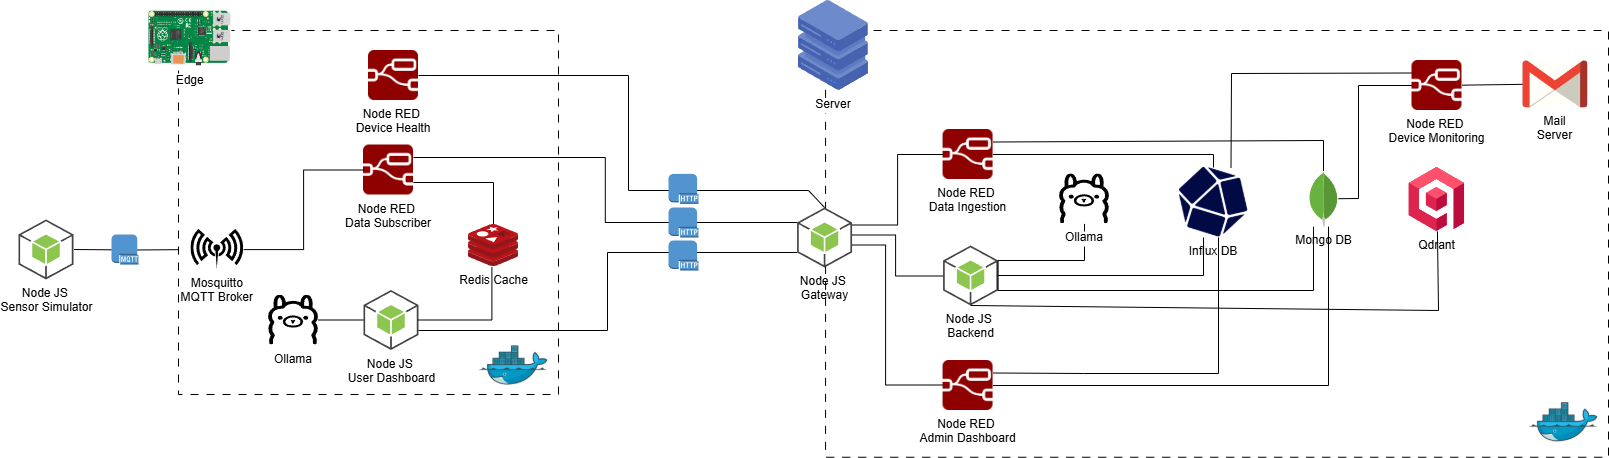
\includegraphics[width=1.3\textwidth]{arichitecture.png}}
\caption{Hybrid Architecture Overview}
\label{fig:architecture}
\end{figure}

\section{Edge Tier: Local Processing and Ingestion}
The Edge Tier is the platform's first processing layer. It handles high-frequency data acquisition, local validation, and patient interaction. Sensor readings are filtered and cached locally for immediate use while also being forwarded to the cloud. The patient dashboard continues to display locally cached measurements when network connectivity is unavailable. Cloud-dependent RAG responses, however, require connectivity. The tier comprises the following components:

\begin{itemize}
\item \textbf{Node.js Sensor Simulator:} Generates synthetic vital sign data to model clinical scenarios, including healthy baselines and critical events such as cardiac arrest.
\item \textbf{Mosquitto MQTT Broker:} Receives data published by the sensor simulator and distributes them to downstream subscribers.
\item \textbf{Node-RED Device Health Flow:} Monitors the operational status of connected sensors and devices, detecting and reporting faults or connectivity anomalies.
\item \textbf{Node-RED Data Subscriber Flow:} Subscribes to the MQTT telemetry stream, validates incoming packets, and forwards them both to the local Redis cache and to the cloud gateway.
\item \textbf{Redis Cache:} Provides state management for vital signs, ensuring that the most recent physiological readings are immediately available to the local dashboard.
\item \textbf{Node.js User Dashboard:} Displays real-time patient vitals and exposes the AI assistant chat interface. It reads from the local Redis cache so that vital-sign monitoring remains available offline.
\item \textbf{Local Ollama Instance:} Executes a local LLM at the edge to perform intent detection, acting as a safety gatekeeper that determines whether a user query is clinically relevant before escalating it to the cloud, thereby reducing latency and filtering unsafe or out-of-scope requests.
\end{itemize}

This arrangement enables continued local monitoring during periods of network unavailability, although cloud-hosted assistant functions are temporarily unavailable.

\section{Cloud Tier: Centralized Intelligence}
The Cloud Tier hosts the computationally intensive and stateful parts of the platform. It receives validated telemetry from the edge and stores it in specialized databases for trend analysis and clinical review. It also exposes the REST API, executes the complete RAG pipeline, and coordinates device monitoring and alert notifications. The tier comprises the following components:

\begin{itemize}
\item \textbf{Node.js Gateway:} Serves as the central entry point for edge-to-cloud communication over HTTPS and performs request validation and traffic routing.
\item \textbf{Node.js Backend:} Implements the application logic and exposes the REST API consumed by the dashboards and AI assistant.
\item \textbf{Node-RED Data Ingestion:} Standardizes incoming telemetry streams from the edge before committing them to the time-series database.
\item \textbf{Node-RED Device Monitoring:} Orchestrates the device health-state tracking flow and triggers alert notifications when anomalous conditions are detected.
\item \textbf{Node-RED Admin Dashboard:} Provides a dedicated monitoring interface for system administrators, enabling real-time visibility into data flows and service health.
\item \textbf{Ollama Instance:} Hosts the full-capacity LLM for complex clinical reasoning and RAG-based response generation.
\item \textbf{InfluxDB:} Time-series database for the long-term persistence of high-frequency sensor vitals, enabling trend analysis and historical review by clinical experts.
\item \textbf{MongoDB:} Document-oriented database for application metadata, user profiles, and clinical session records.
\item \textbf{Qdrant:} Vector search engine that indexes medical document embeddings, enabling semantic retrieval for the RAG pipeline.
\end{itemize}


\section{System Workflows}
The platform coordinates three main workflows across the two tiers: IoT telemetry ingestion, document-based RAG, and RAG enriched with rule-based analysis.

\subsection{IoT Data Ingestion Workflow}
Sensor telemetry is collected and validated at the edge before being forwarded to the cloud for persistent storage. Validation at both tiers reduces the likelihood that malformed measurements reach the time-series database.

\begin{figure}[H]
\centering
\includegraphics[width=1.0\textwidth]{iotFlow.png}
\caption{IoT Data Ingestion Flow}
\label{fig:iotflow}
\end{figure}

\begin{itemize}
\item \textbf{Data Generation:} The Sensor Simulator publishes synthetic vital sign telemetry over MQTT.
\item \textbf{Edge Subscription and Validation:} The Node-RED Data Subscriber flow captures incoming packets, applies validation rules, and caches valid readings in Redis for immediate dashboard use.
\item \textbf{Cloud Forwarding:} Validated packets are transmitted via HTTPS to the Cloud Gateway.
\item \textbf{Cloud Ingestion and Validation:} The server-side Node-RED flow applies a secondary validation pass to enforce data integrity before persistence.
\item \textbf{Persistent Storage:} Clean data is committed to InfluxDB for long-term trend analysis and clinical review.
\end{itemize}

\subsection{AI Assistant and RAG Pipeline}
This workflow implements a conventional document-based RAG pipeline. Its knowledge base consists of biomedical reference texts indexed in Qdrant. The pipeline does not analyze live sensor data; it answers patient queries by retrieving relevant passages and placing them in the generation context. Queries are first screened at the edge for clinical relevance and are then routed to the cloud for retrieval and generation. This separation is important: RAG improves the informational basis of an answer, but it does not independently establish the patient's current clinical state.

\begin{figure}[H]
\centering
\makebox[\textwidth][c]{\includegraphics[width=1.3\textwidth]{chatFlow.png}}
\caption{RAG Pipeline Flow}
\label{fig:chatflow}
\end{figure}

\begin{itemize}
\item \textbf{Intent Detection (Edge):} The local edge Ollama instance acts as a safety gatekeeper, confirming the query is clinically relevant before it is escalated to the cloud.
\item \textbf{Query Rephrasing (Cloud):} The query is rewritten to improve semantic matching against the indexed documents.
\item \textbf{Document Retrieval:} Qdrant returns the most relevant text fragments from the pre-loaded biomedical knowledge base.
\item \textbf{LLM Invocation:} The cloud Ollama instance generates a response conditioned on the retrieved passages and the patient's original query.
\item \textbf{Answer Delivery:} The grounded response is streamed to the patient dashboard.
\end{itemize}

\subsection{Rule-Based Diagnosis Workflow}
This workflow extends the document-based pipeline with a deterministic diagnosis block executed before LLM invocation. The block aggregates sensor measurements over a configurable trailing window, set to five minutes in the prototype, and computes the minimum, maximum, and mean for each metric. Aggregation reduces the influence of isolated fluctuations while retaining a recent view of the simulated patient's state. A rule engine compares these statistics with configured clinical thresholds and assigns a structured label, such as \textit{Tachyarrhythmia} or \textit{Hypoxemia}. The label and retrieved passages are combined in an enriched prompt. The model therefore receives both explanatory biomedical material and a concise representation of recent measurements. These labels are decision-support inputs within the prototype and should not be interpreted as clinically validated diagnoses.

\begin{figure}[H]
\centering
\makebox[\textwidth][c]{\includegraphics[width=1.3\textwidth]{dataAnalystFlow.png}}
\caption{Data Analyst and Rule-Based Diagnosis Flow}
\label{fig:dataanalystflow}
\end{figure}

\begin{itemize}
\item \textbf{Intent Detection (Edge):} As in the standard RAG pipeline, the local Ollama instance screens the query for clinical relevance before escalation.
\item \textbf{Query Rephrasing (Cloud):} The query is rewritten to improve semantic matching against the indexed documents.
\item \textbf{Vitals Aggregation:} In parallel, sensor readings from the last five minutes are retrieved from InfluxDB and summarized into min, max, and mean values per metric.
\item \textbf{Diagnosis Labeling:} The rule engine evaluates the aggregated statistics against configured reference ranges and assigns a structured label with severity metadata.
\item \textbf{Document Retrieval:} Qdrant returns the most relevant text fragments from the pre-loaded biomedical knowledge base.
\item \textbf{Data Analysis Prompt:} The diagnosis label and the retrieved passages are combined into a single enriched prompt for the LLM.
\item \textbf{LLM Invocation and Answer Delivery:} The cloud Ollama instance generates a response conditioned on both sources and streams it back to the patient dashboard.
\end{itemize}

\section{Clinical Dashboard and Simulation Analysis}
The platform provides two interfaces for distinct roles: a patient dashboard at the edge and an expert dashboard in the cloud.

\subsection{Patient Dashboard}
The Patient Dashboard is the primary interface for the monitored patient. It reads vital signs directly from the local Redis cache and displays heart rate, blood pressure, oxygen saturation, and respiratory rate even when cloud connectivity is lost. When the cloud is reachable, the same interface provides access to the AI assistant and its RAG-generated responses.

\begin{figure}[H]
\centering
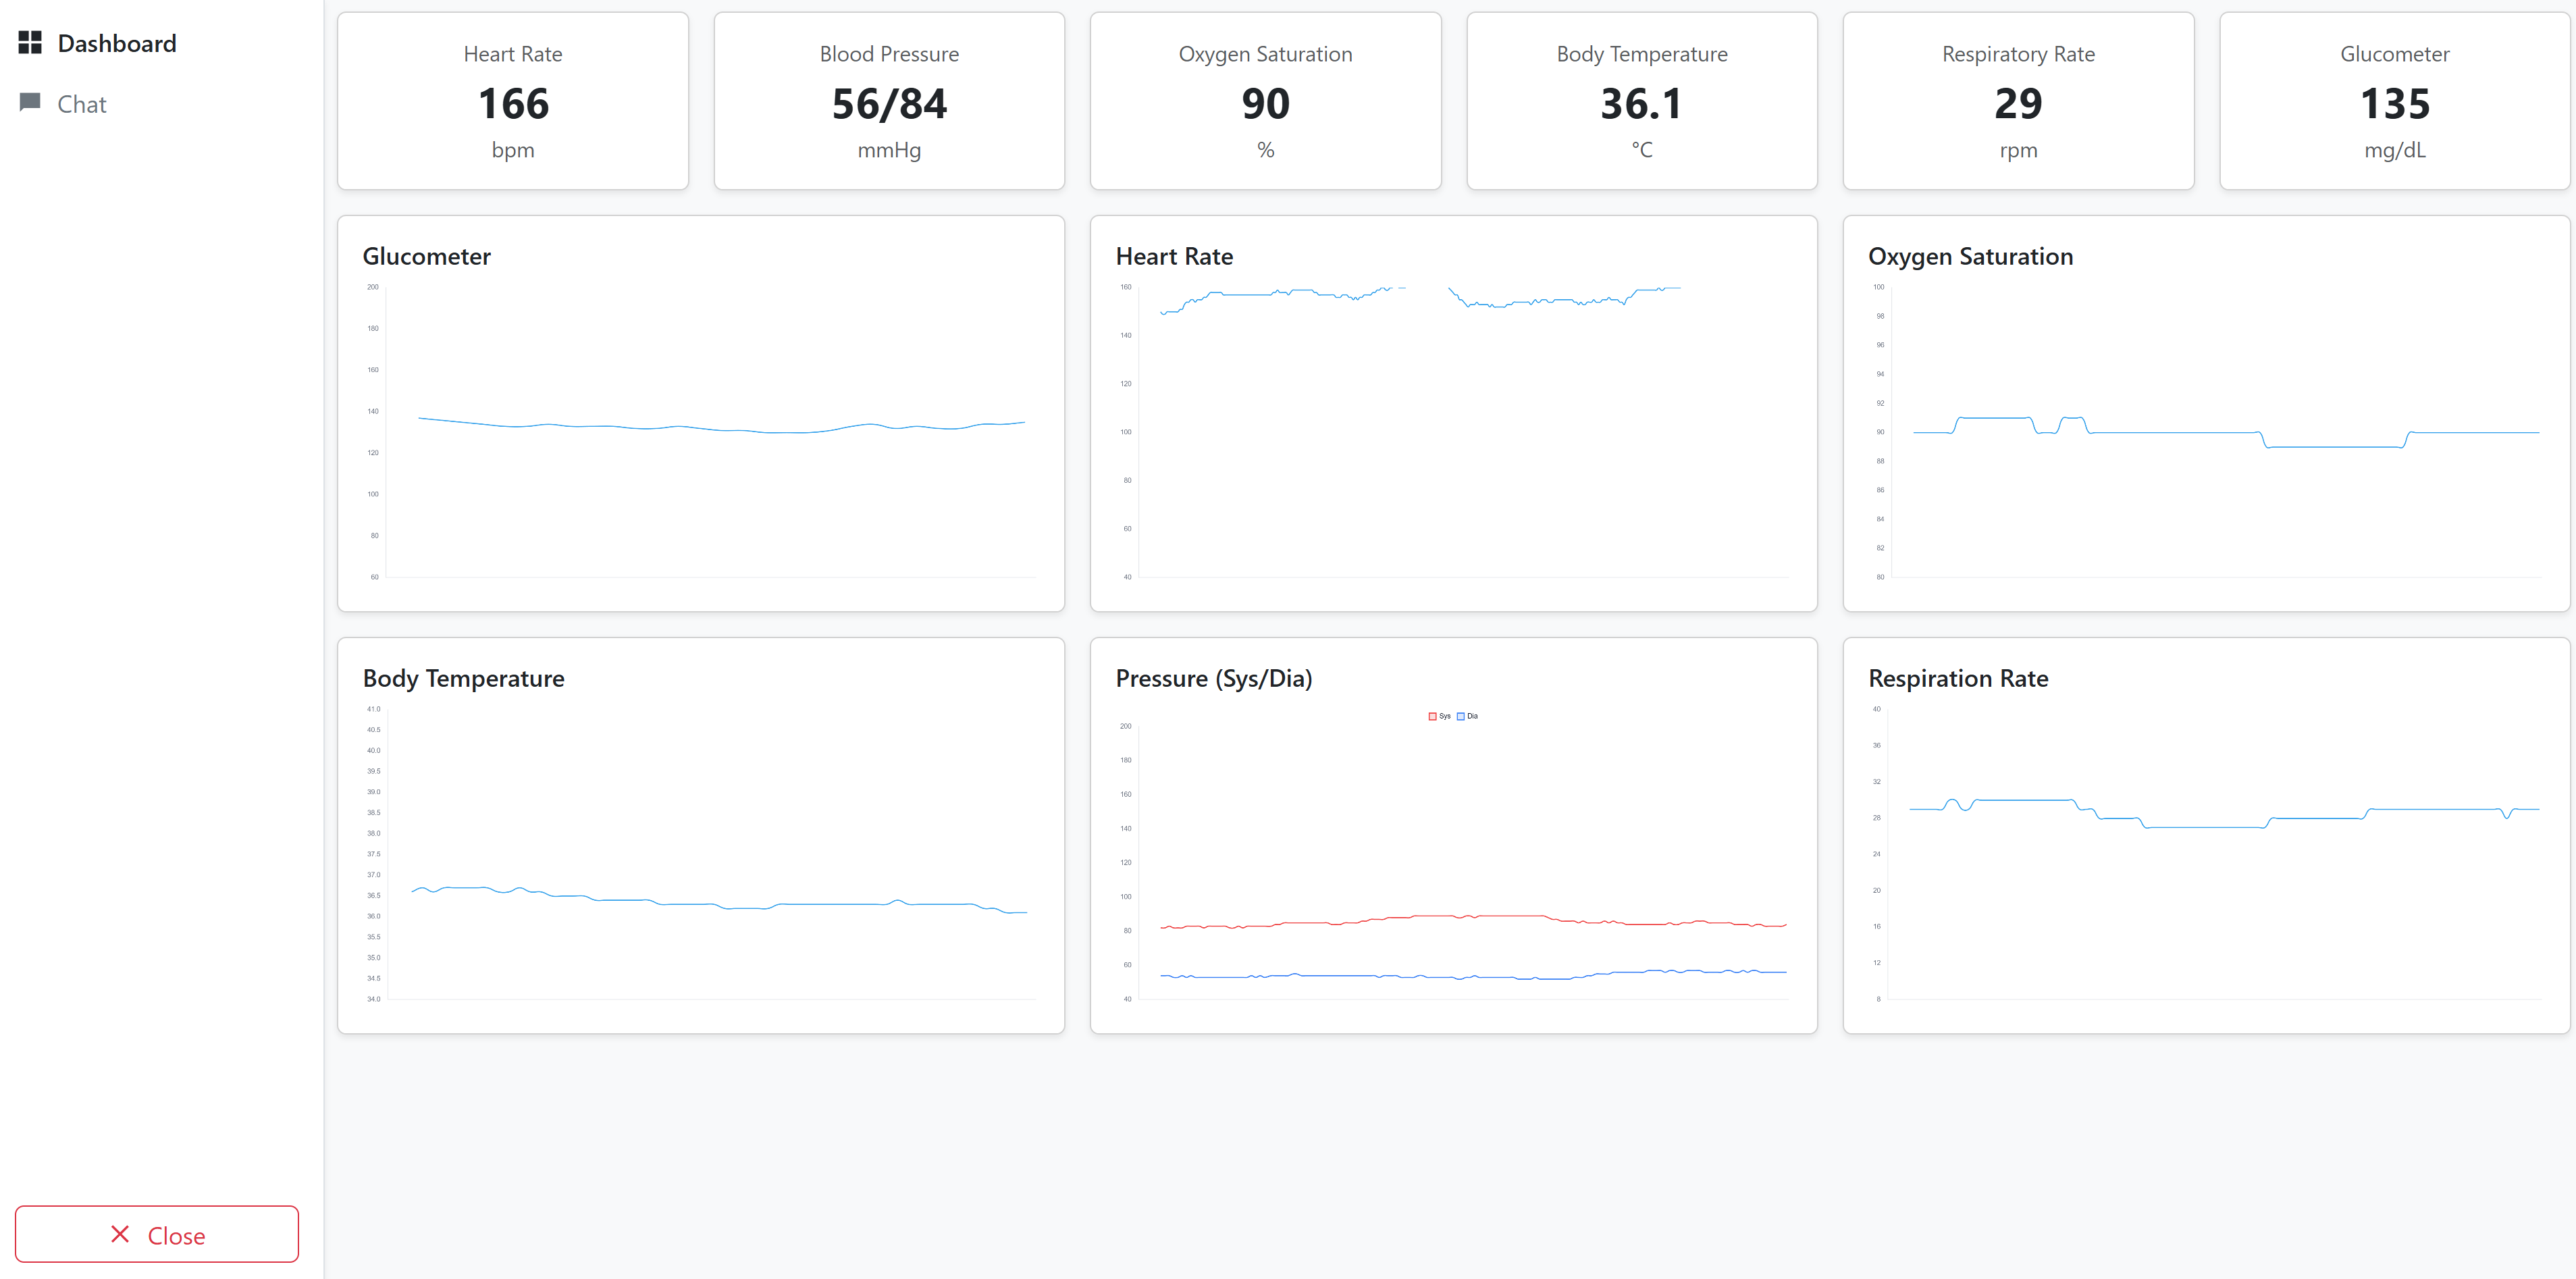
\includegraphics[width=1.0\textwidth]{patient-dashboard.png}
\caption{Patient Dashboard: Vitals Visualization}
\label{fig:patient_dashboard}
\end{figure}

\begin{figure}[H]
\centering
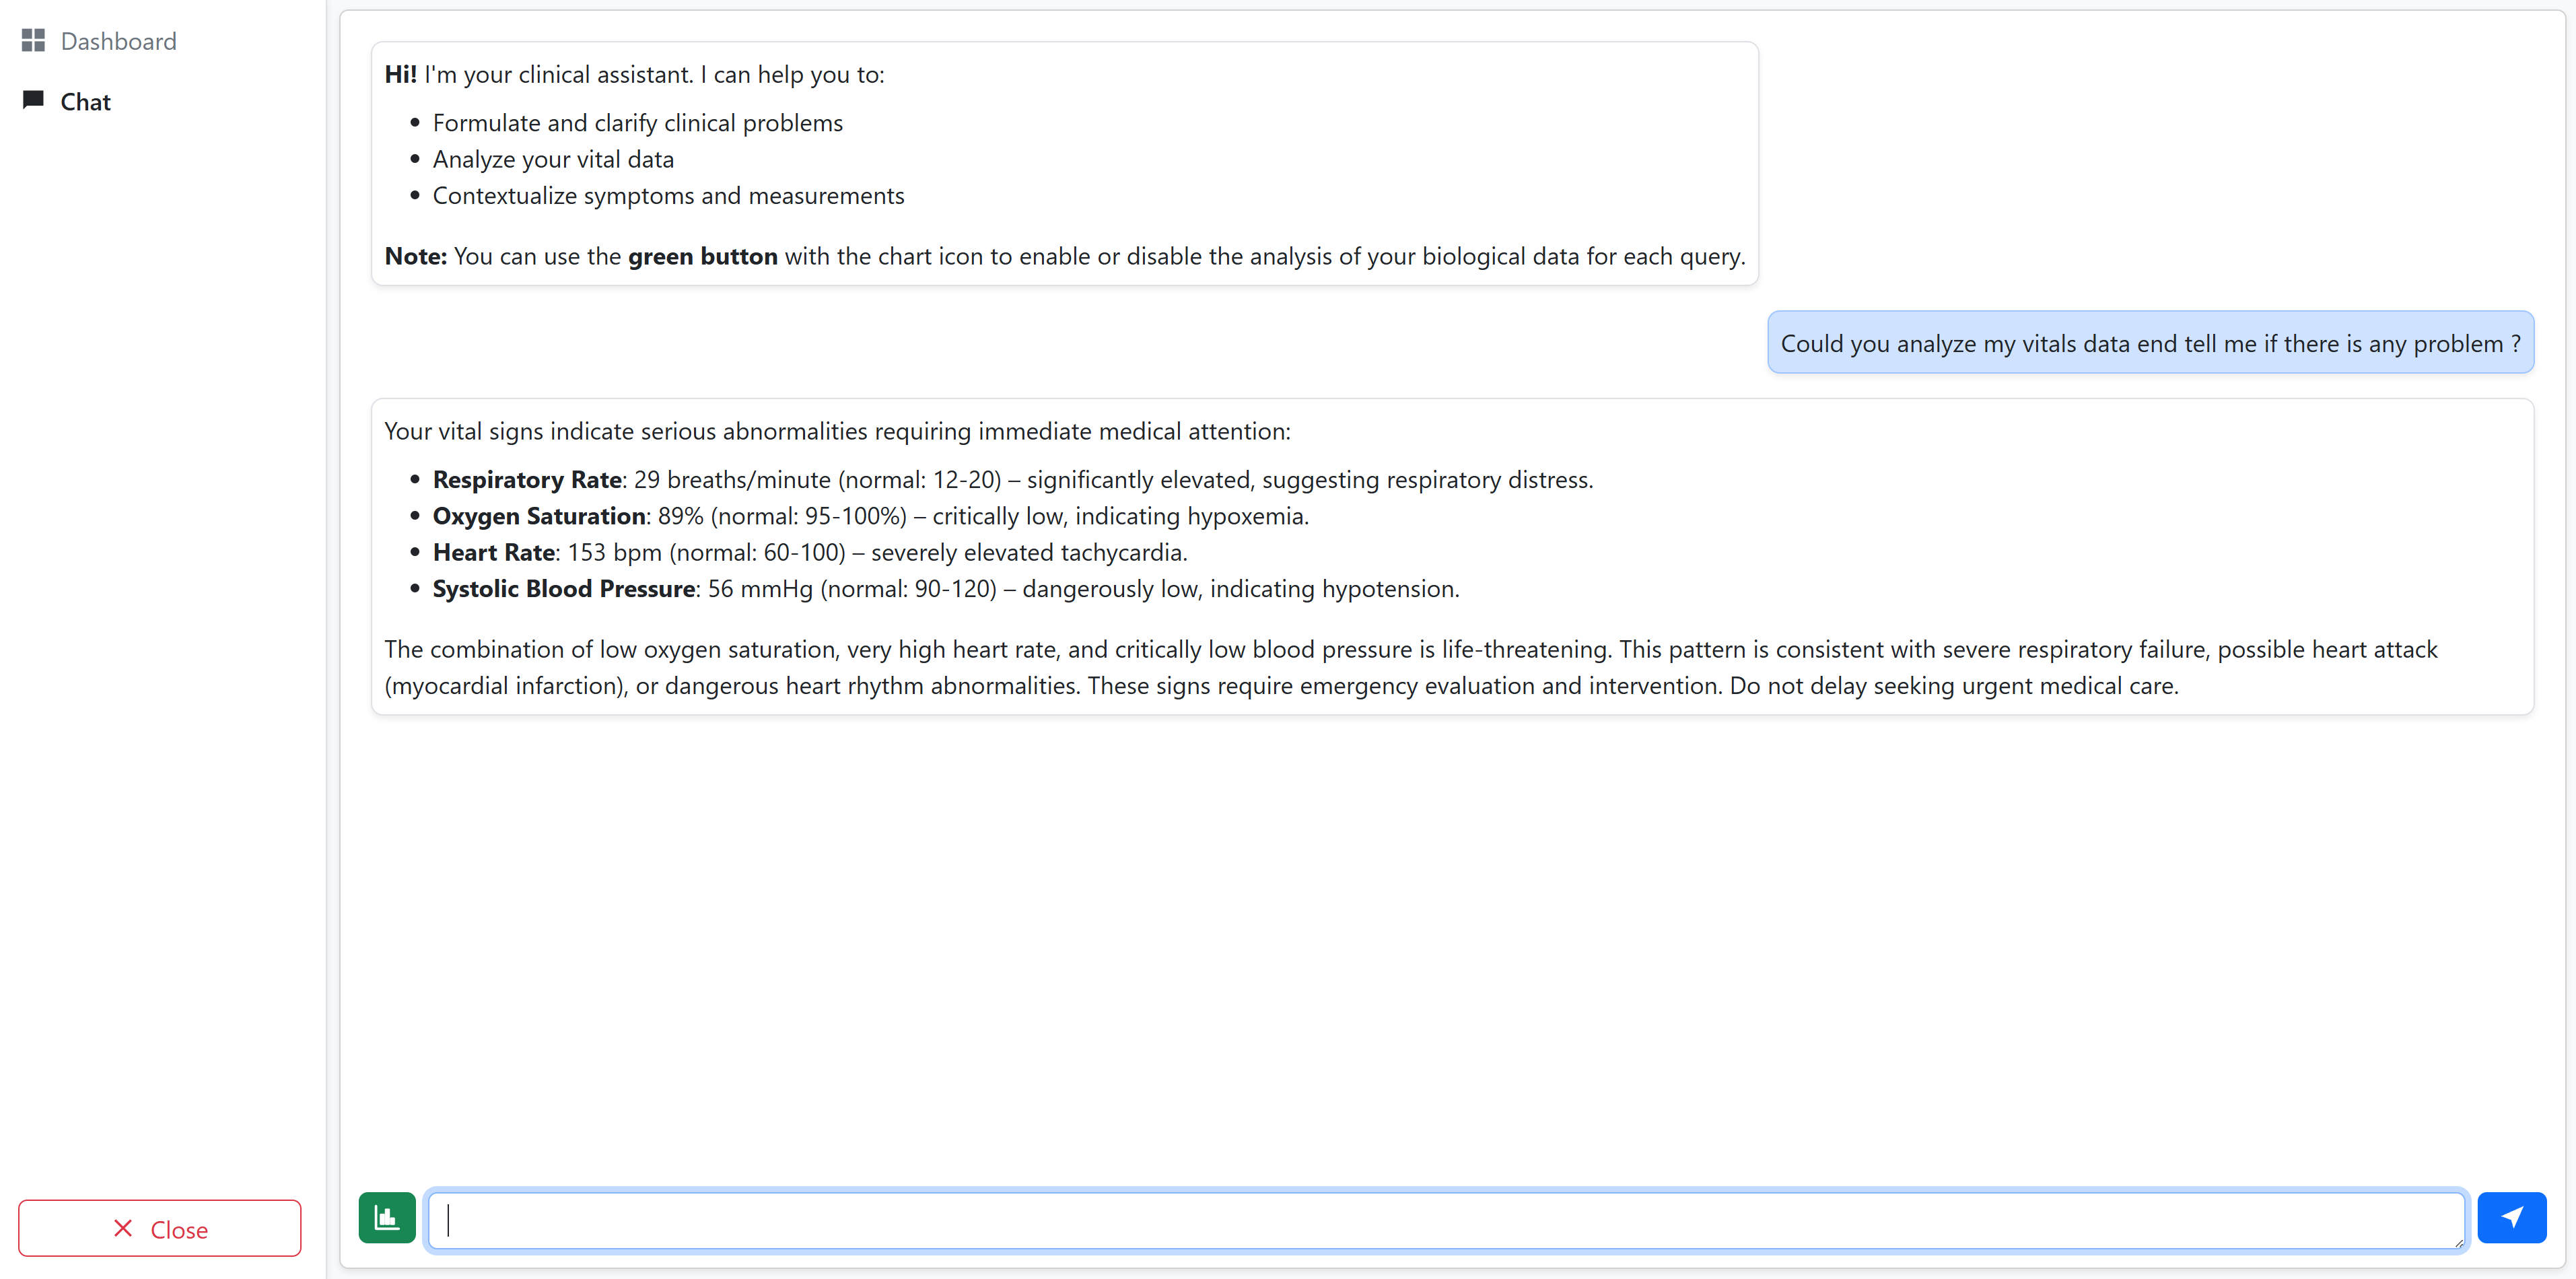
\includegraphics[width=1.0\textwidth]{patient-chat.png}
\caption{Patient Dashboard: AI Assistant Chat Interface}
\label{fig:patient_chat}
\end{figure}

\subsection{Expert Dashboard}
The Expert Dashboard supports healthcare professionals and system administrators. It contains a device panel showing registered edge nodes and their connectivity status, a panel for active and historical monitoring sessions, and a detailed view with live vital signs and interaction history for a selected patient. Together, these views provide a centralized overview of multiple edge nodes and highlight conditions flagged by the monitoring logic.

\begin{figure}[H]
\centering
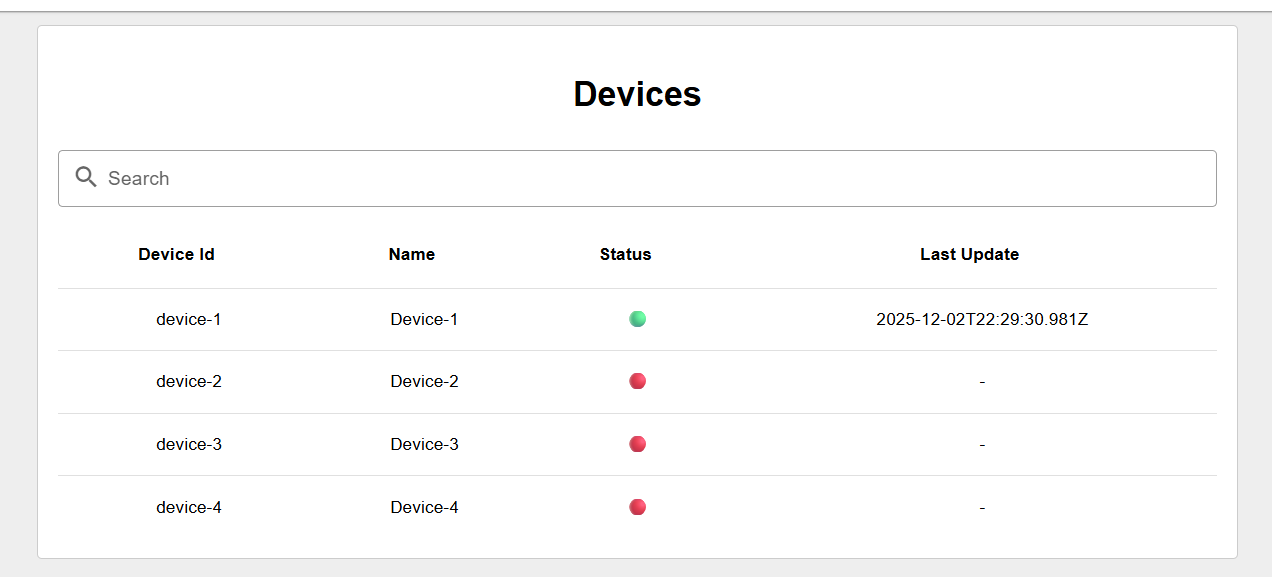
\includegraphics[width=0.8\textwidth]{expert-devices-list.png}
\caption{Expert Dashboard: Devices Telemetry}
\label{fig:expert_devices}
\end{figure}

\begin{figure}[H]
\centering
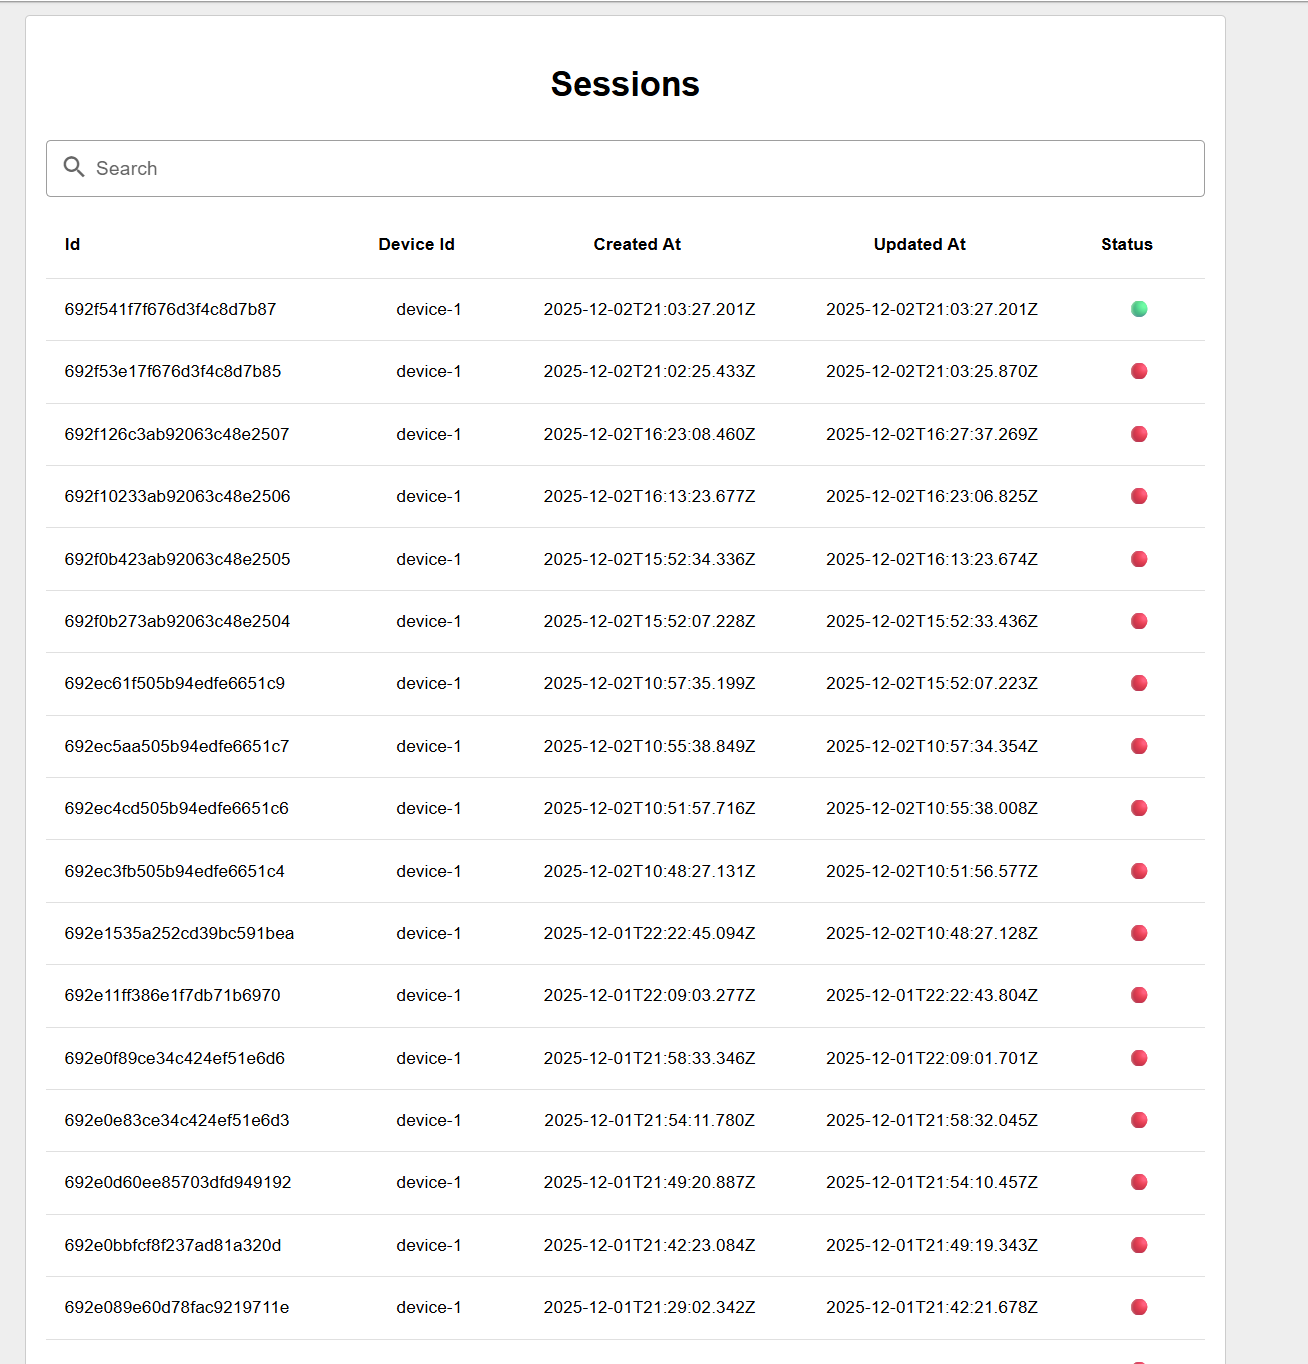
\includegraphics[width=0.8\textwidth]{expert-sessions-list.png}
\caption{Expert Dashboard: Active Sessions List}
\label{fig:expert_sessions}
\end{figure}

\begin{figure}[H]
\centering
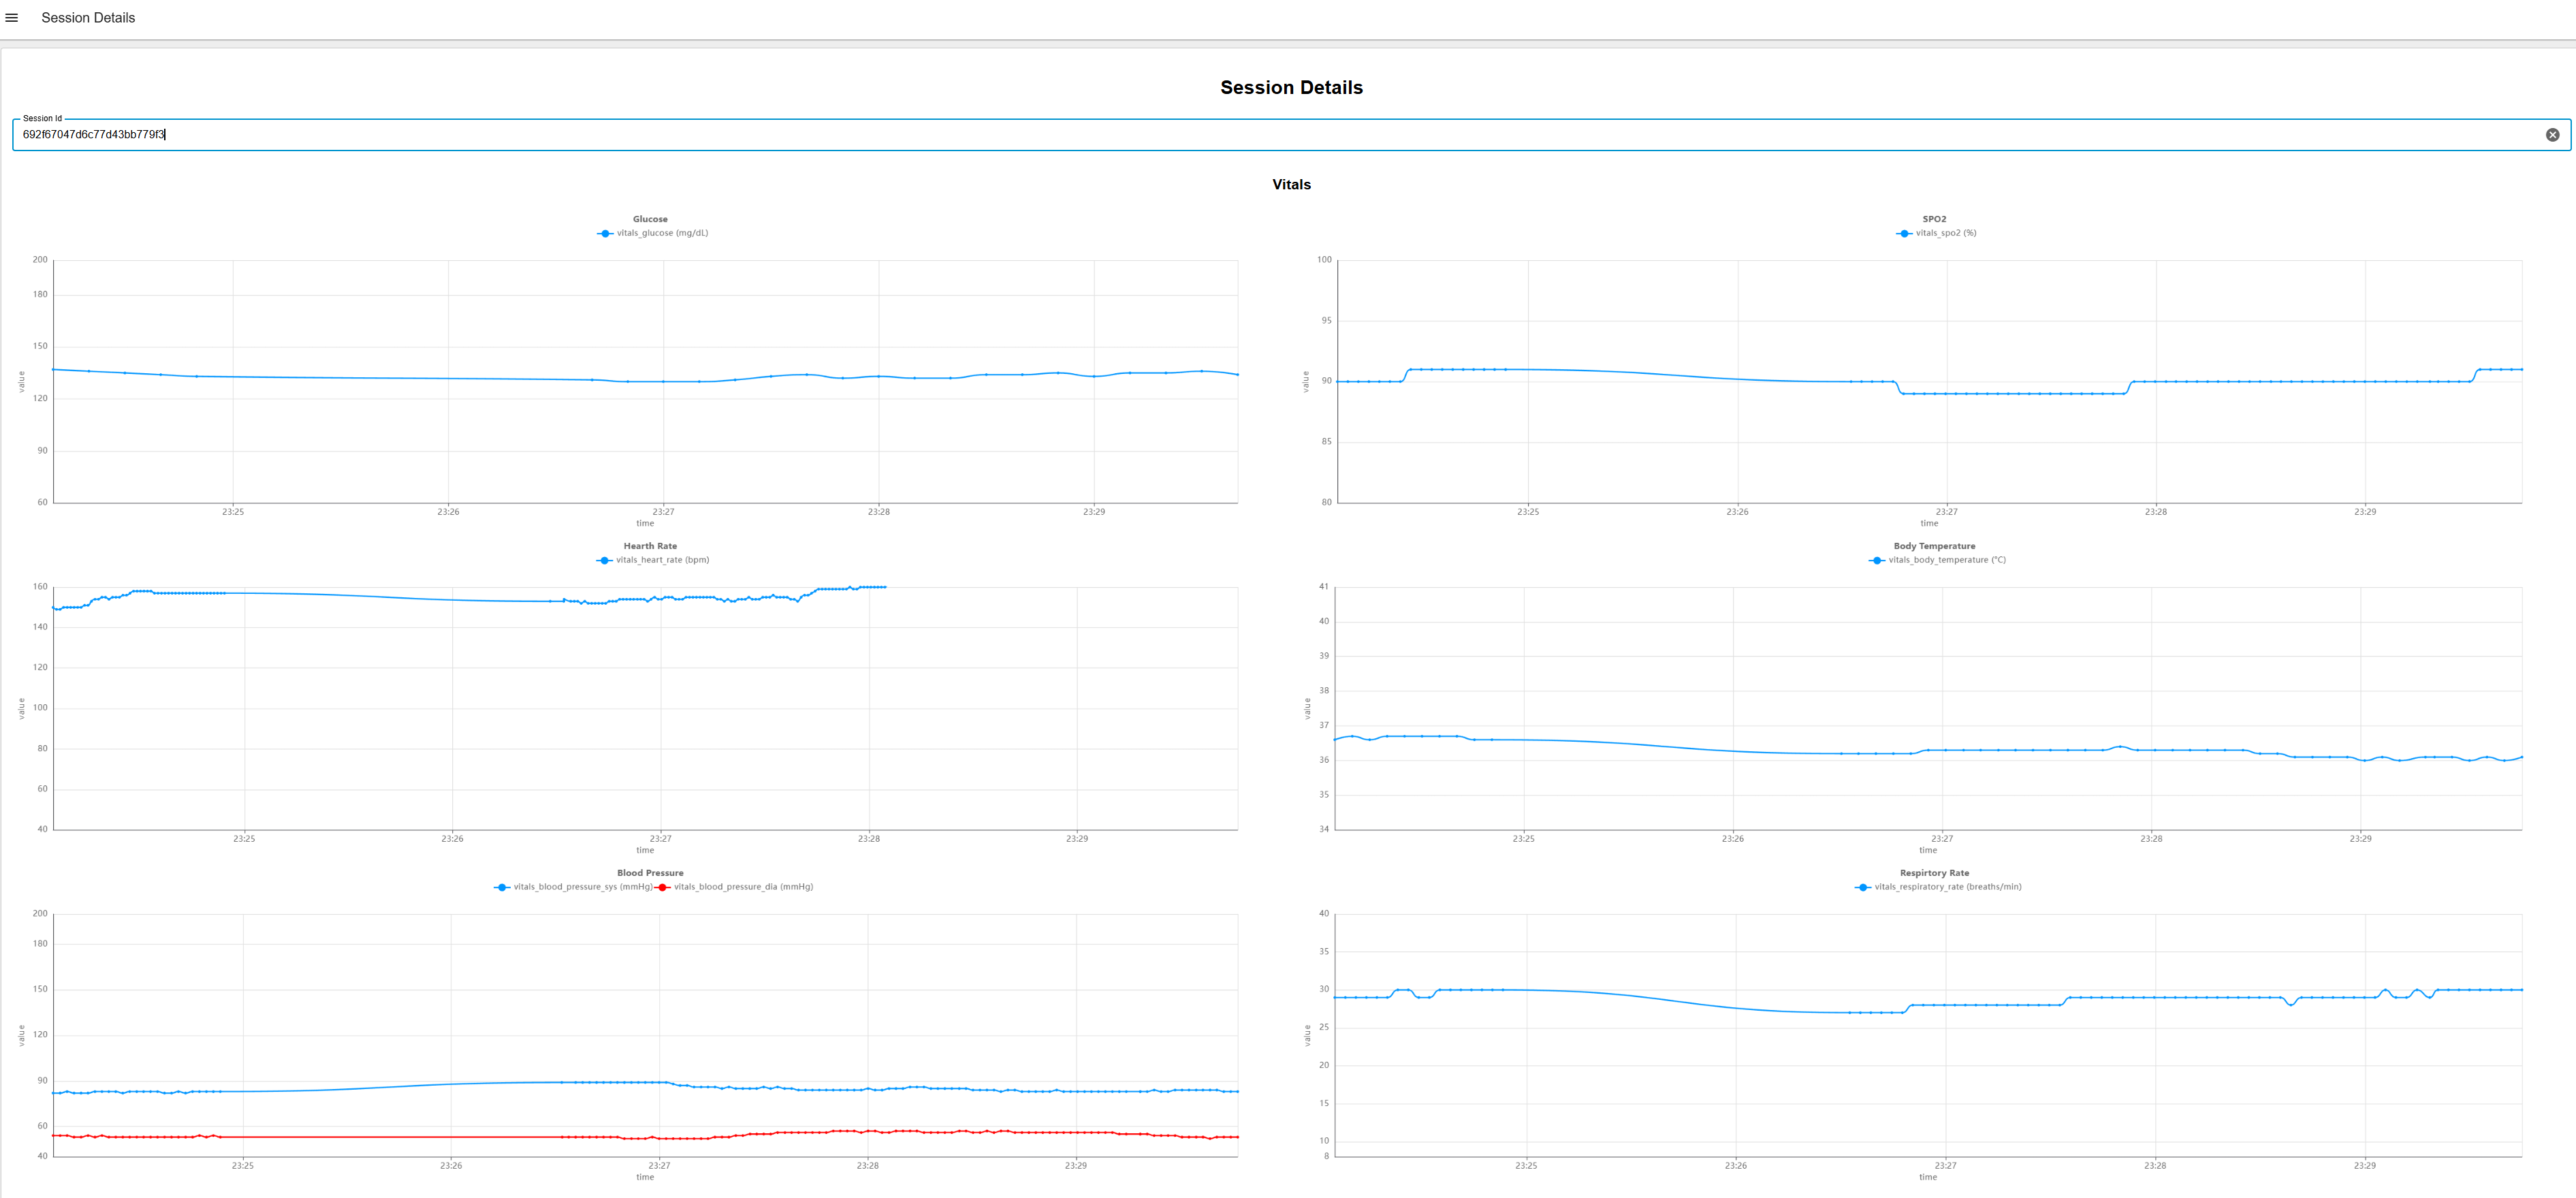
\includegraphics[width=1.0\textwidth]{expert-session-details.png}
\caption{Expert Dashboard: Detailed Session Vitals}
\label{fig:expert_session_details}
\end{figure}

\section{Limitations and Future Work}
The prototype currently uses simulated sensor data, a single deployed edge node, deterministic thresholds, and a biomedical corpus that is indexed offline. Its response quality has been assessed qualitatively during development, but no controlled comparison of RAG and non-RAG outputs or evaluation with clinicians has yet been conducted. Security, privacy, failure recovery, and performance under concurrent multi-patient workloads also require systematic evaluation. Future work will therefore consider the following directions:

\begin{itemize}
\item \textbf{Quantitative RAG Evaluation:} Compare answers generated with and without retrieval using measures of relevance, factual consistency, source support, latency, and clinician judgment.
\item \textbf{Knowledge-Base Maintenance:} Introduce document provenance, versioning, and update procedures so that retrieved medical information remains traceable and current.
\item \textbf{Graph RAG:} Evaluate knowledge graphs for representing and retrieving relationships that are difficult to capture through vector similarity alone.
\item \textbf{Diagnostic Models:} Compare the current rule-based component with validated machine-learning approaches while retaining interpretable safety constraints.
\item \textbf{Real Devices and Clinical Validation:} Integrate certified medical devices and conduct appropriately supervised studies in realistic settings.
\item \textbf{Security and Privacy:} Add authentication, authorization, encryption, auditing, and data-governance controls appropriate for health information.
\item \textbf{Scalability and Resilience:} Evaluate container orchestration, high availability, and failure recovery under concurrent multi-patient workloads.
\end{itemize}

\section{Conclusion}
This paper presented a hybrid edge--cloud platform for real-time health monitoring and AI-assisted patient interaction. The edge tier validates and caches telemetry, supports continuous local visualization, and screens user queries. The cloud tier stores historical data, provides centralized supervision, and executes two assistant workflows: document-based RAG and an enriched variant that also incorporates rule-based summaries of recent vital signs.

The prototype indicates that retrieval can improve response quality by giving the language model relevant biomedical context instead of relying exclusively on knowledge encoded in its parameters. In the enriched workflow, the deterministic diagnosis block further aligns the response with recent sensor observations. The principal benefit of RAG in this system is therefore not autonomous diagnosis, but better-grounded and more contextually relevant communication. This distinction is particularly important in a health-monitoring setting, where fluent output alone is insufficient evidence of correctness.

The work also identifies clear limits. The current implementation relies on simulated data and qualitative observations, and it has not undergone clinical validation or a controlled evaluation of response quality. The results should consequently be interpreted as evidence of architectural feasibility rather than clinical effectiveness. Future experiments should compare RAG and non-RAG responses, assess source attribution and factual consistency, measure end-to-end latency, and involve qualified clinical reviewers. Within these boundaries, the architecture provides a practical basis for studying how retrieval, streaming telemetry, and deterministic analysis can complement one another in remote health-assistance systems.
\end{document}
